%%================================================
%% Appendix A
%%================================================
\chapter{คู่มือการติดตั้งและการใช้งาน}
\label{appA}
\section{วิธีการใช้งานบน Docker}
\raggedright ขั้นตอนแรกให้ทําการสร้างไดเรกทอรีเพื่อเก็บไฟล์ และ ทำการเข้าไปในไดเรกเทอรี ด้วยคำสั่ง
\begin{lstlisting}
cd directory
\end{lstlisting}
จากนั้นทำการสร้าง docker images ด้วยคำสั่ง 
\begin{lstlisting}
docker-compose build
\end{lstlisting}
เปิดใช้งาน container ของ Docker ด้วยคําสั่ง
\begin{lstlisting}
docker-compose up
\end{lstlisting}
สามารถดูสถานะของ container ด้วยคำสั่ง
\begin{lstlisting}
docker-compose ps
\end{lstlisting}

\section{วิธีการใช้งานบนเครื่อง (Local)}

\raggedright ขั้นตอนแรกให้ทําการสร้างไดเรกทอรีเพื่อเก็บไฟล์ และ ทำการเข้าไปในไดเรกเทอรี ด้วยคำสั่ง
\begin{lstlisting}
cd directory
\end{lstlisting}
หลังจากนั้นทำการ runserver ของ API ด้วยคำสั่ง 
\begin{lstlisting}
go run main.go
\end{lstlisting}

โดย API ดังกล่าวนั้นสามารถทดสอบได้โดยการใช้โปรแกรมที่สามารถส่ง request เพื่อทดสอบ เช่น Postman

\section{วิธีการส่ง request API}
\raggedright API มีจํานวนทั้งหมด 2 ตัว

\begin{itemize}[\textbullet]
    \item compile API ใช้สำหรับ compile และ รันโปรแกรมเพื่อส่งผลลัพธ์ออกมา
    \item problem API ใช้ในการตรวจผลลัพธ์ของ source code
\end{itemize}

\raggedright โดยที่จะส่ง API ไปที่ endpoint compile/ และ problem/  ซึ่ง API แต่ละเส้นมี request ดังนี้

\begin{enumerate}
    \item compile API มีจํานวน field ทั้งหมด 3 field
        \begin{enumerate}
            \item source 
            \item language 
            \item input 
        \end{enumerate} 
        
        \begin{figure}[H]
            \centering
                \centering
                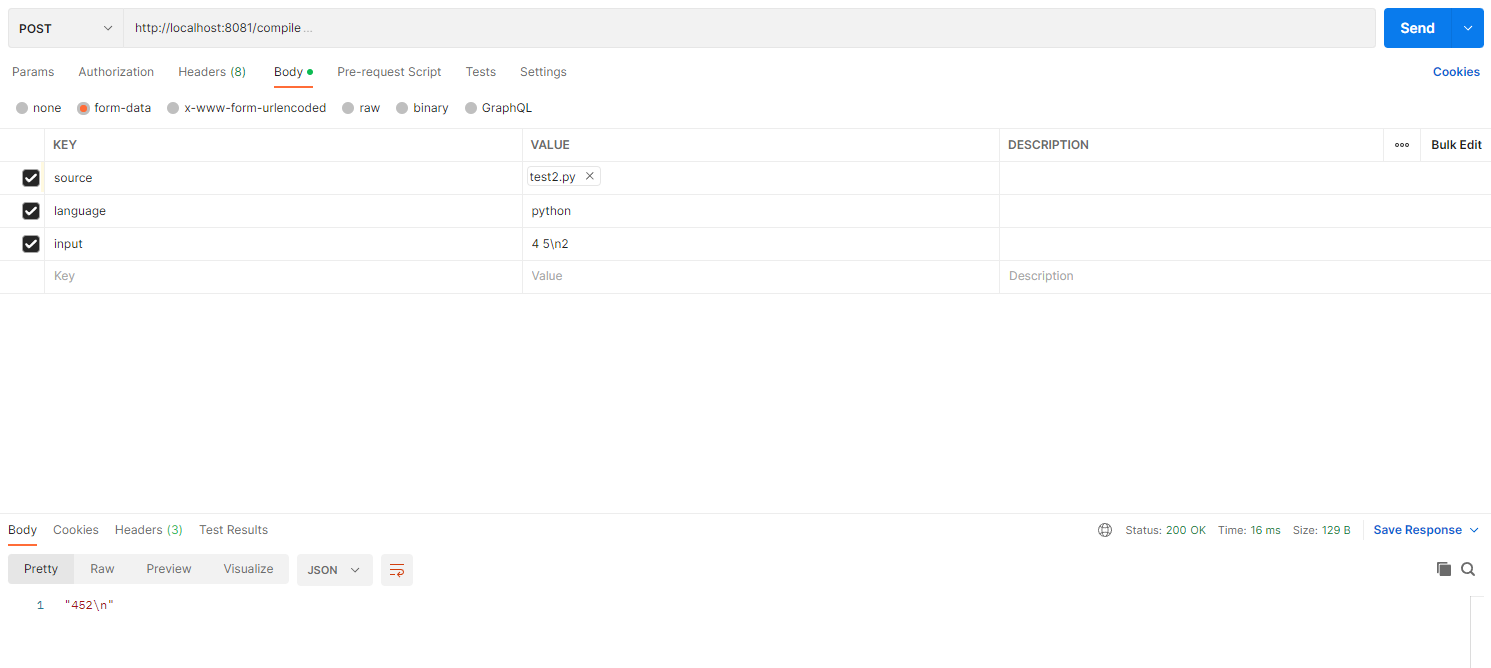
\includegraphics[width=5in]{latex/figures/compileAPI.png}
            \caption{ตัวอย่างการใช้ compile API ด้วยโปรแกรม Postman}
        \end{figure}
        
    \item problem API มีจํานวน field ทั้งหมด 4 field
        \begin{enumerate}
            \item problem file 
            \item answer file
            \item language 
            \item input
        \end{enumerate}
        
        \begin{figure}[H]
            \centering
                \centering
                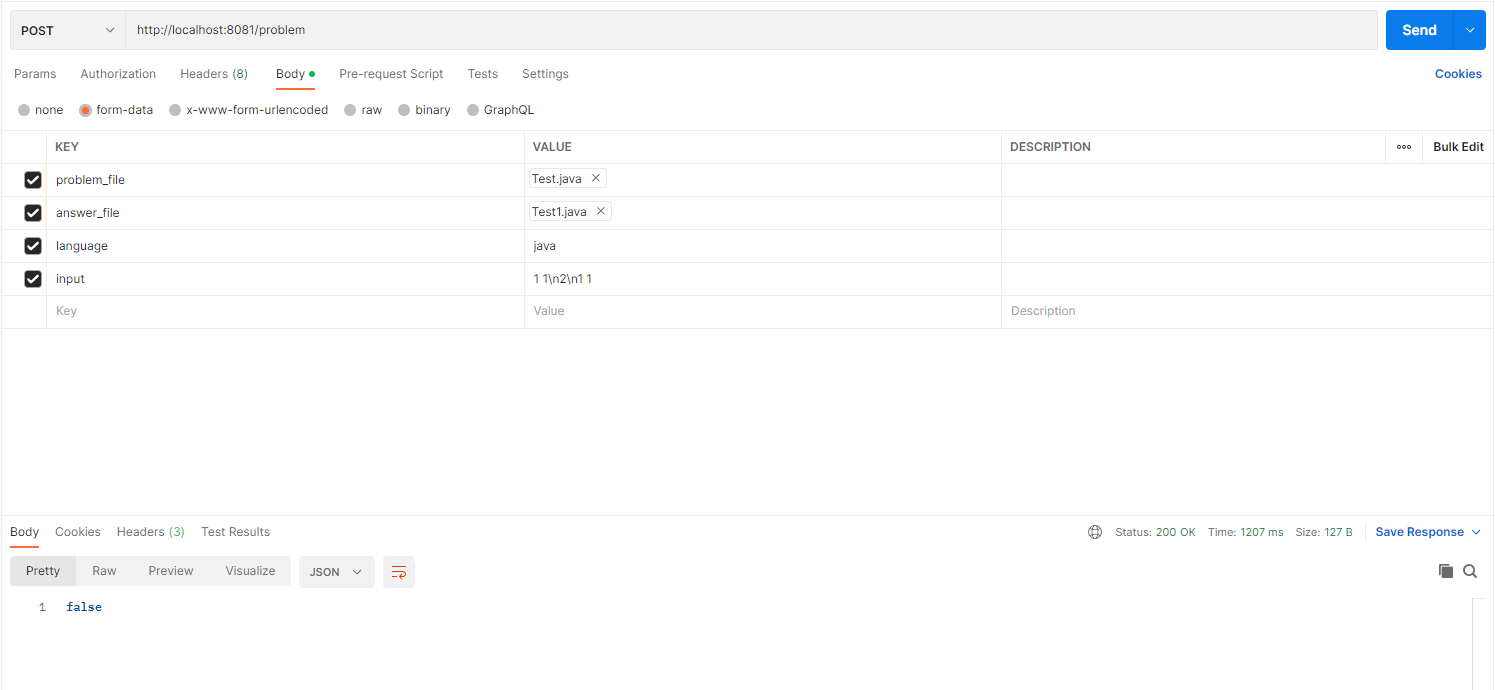
\includegraphics[width=5in]{latex/figures/problemAPI.png}
            \caption{ตัวอย่างการใช้ problem API ด้วยโปรแกรม Postman}
        \end{figure}
\end{enumerate}

        